\subsection*{(i) Original RiverSwim MDP}
I implemented a certainty-equivalence off-policy optimization (CE-OPO) approach in the RiverSwim environment. 
I used an $\epsilon$-greedy behavior policy (with $\epsilon=0.15$) to gather samples and periodically updated 
my estimates of the transition probabilities and rewards. I then ran Value Iteration (VI) on the estimated MDP 
to obtain an approximate $Q$-function. 

Because running VI at every single step (up to $10^6$) was computationally expensive on my machine, I chose to 
call VI every 1000 steps instead. This allowed me to keep a large horizon (on the order of $10^6$ steps) without 
overheating my computer. The figure below shows the evolution of three performance metrics for the \emph{original} 
RiverSwim environment:

\begin{figure}[H]
    \centering
    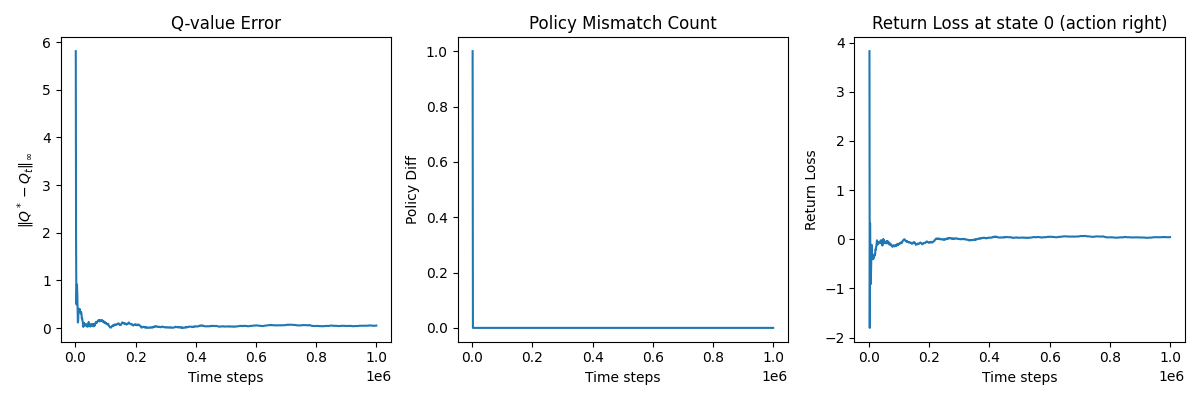
\includegraphics[width=1\textwidth]{Code/RiverSwim_CE-OPO.png}
    \caption{Performance metrics in the original RiverSwim MDP: (left) $Q$-value error $\|Q^* - Q_t\|_\infty$, 
    (middle) policy mismatch count, and (right) return loss at state 0 (action = right).}
    \label{fig:original}
\end{figure}

\subsection*{(ii) Variant RiverSwim MDP}
I also tested a variant of RiverSwim in which taking the action ``right'' in the rightmost state 
(index \texttt{nS-1}) yields a reward drawn uniformly at random from $[0,2]$. Below is the snippet of my modified 
\texttt{step} function for this variant:

\begin{lstlisting}[language=Python, caption={Definition of the variant\_step function.}, basicstyle=\ttfamily\small]
    def variant_step(self, action):
        # If in the rightmost state (nS-1) and taking action 'right' (1):
        if self.s == self.nS - 1 and action == 1:
            reward = np.random.uniform(0, 2)
        else:
            reward = self.R[self.s, action]
        new_s = np.random.choice(np.arange(self.nS), p=self.P[self.s, action])
        self.s = new_s
        return new_s, reward
\end{lstlisting}

In order to evaluate the true $Q$-function in this variant, I set the expected reward of that random transition 
to $1$ in the ``true'' reward matrix. I then ran the same CE-OPO procedure (again calling VI every 1000 steps). 
Figure~\ref{fig:variant} shows the corresponding performance metrics:

\begin{figure}[H]
    \centering
    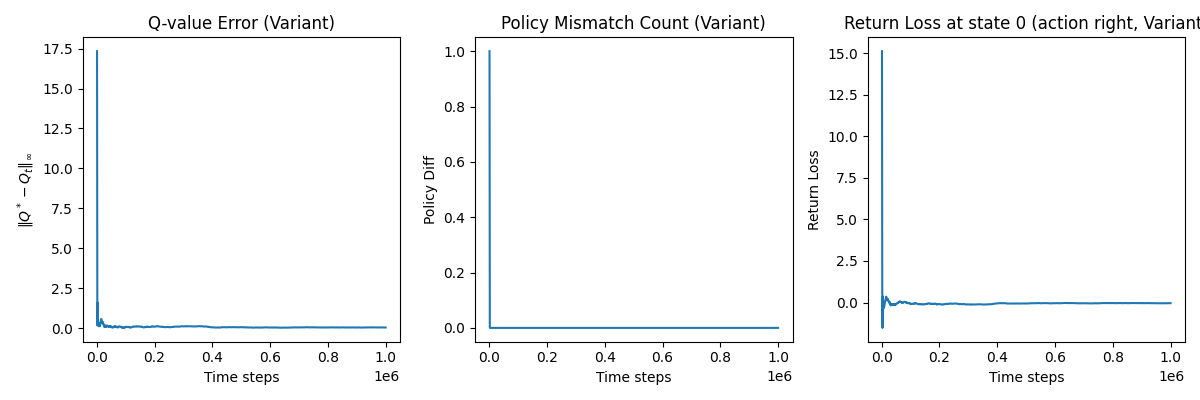
\includegraphics[width=1\textwidth]{Code/RiverSwim_CE-OPO_Variant.png}
    \caption{Performance metrics in the variant RiverSwim MDP, where the reward for action = right 
    in the rightmost state is drawn from $\mathrm{Unif}[0,2]$.}
    \label{fig:variant}
\end{figure}

\subsection*{(iii) Comments and Possible Explanations}
From the two figures, I notice that in both the original and the variant setting, the $Q$-value error $\|Q^*-Q_t\|_\infty$ 
drops quickly within the first portion of the training, then continues to decrease more slowly as time progresses. 
Similarly, the policy mismatch count (i.e., the number of states in which the greedy policy w.r.t. $Q_t$ differs from 
the true optimal policy) quickly goes to zero and remains there, indicating that the estimated policy converges to 
the true one. 

In the variant setting, the randomness in the reward causes a slightly shakier behavior in the Q-value error.
However, the overall performance remains robust, demonstrating that the certainty-equivalence principle effectively
supports off-policy learning in RiverSwim, even under mild stochastic reward modifications.